\section{Evaluation}
\label{sec:eval}

\lstMakeShortInline[mathescape=true]{|}

We have implemented analytic program repair in \toolname: a system for
repairing type errors for a purely functional subset of \ocaml. Next,
we describe our implementation and an evaluation that addresses three
questions:

\begin{itemize}
    \item \textbf{RQ1}: How \emph{accurate} are \toolname's predicted repairs?
                        (\S~\ref{sec:eval:accuracy})
    \item \textbf{RQ2}: How \emph{efficiently} can \toolname synthesize fixes?
                        (\S~\ref{sec:eval:efficiency})
    \item \textbf{RQ3}: How \emph{useful} are \toolname's error messages?
                        (\S~\ref{sec:eval:useful})
    \item \textbf{RQ4}: How \emph{precise} are \toolname's template-directed fixes?

\end{itemize}

% \subsection{Implementation} \label{sec:eval:gen_method}

\mypara{Training Dataset}
%
For our evaluation, we use an \ocaml dataset gathered from an undergraduate
Programming Languages university course, previously used in related work
\citep{yunounderstand,Seidel:2017}. It consists of erroneous programs and their
subsequent fixes and is divided in two parts; the Spring 2014 class (\SPRING)
and the Fall 2015 class (\FALL). The homework required students to write 23
distinct programs that demonstrate a range of functional programming idioms, \eg
higher-order functions and (polymorphic) algebraic data types.

\mypara{Feature Extraction}
%
\toolname represents programs with BOAT vectors over a set of 416 features from
each sub-expression in a program, including:

45 local syntactic features.
%
315 contextual syntactic features. For each subexpression we
additionally extract the local syntactic features of its first 4
(left-to-right) children. In addition, we extract those features for its
ancestors, starting from its parent and going up to two more parent nodes.
    % If an expression does not have a ancestor or children, these features will
    % simply be disabled. If an expression has more than four children, the
    % classifiers will receive no information about the additional children.
    %
88 typing features. We support |int|s, |float|s, |char|s, |string|s, and
    the user-defined |expr|. These features are extracted for each
    sub-expression and its context.
%
1 feature denoting the size of each subexpression.

\mypara{Dataset Cleaning}
%
We extract fixes as expressions replacements over a program pair using \diffsym.
A disadvantage of using \diffsym s with this dataset is that some students may
have made many, potentially unrelated, changes between compilations; at some
point the ``fix'' becomes a ``rewrite''. These rewrites can lead to meaningless
fix templates and error locations. We discard such outliers when the fraction of
subexpressions that have changed in a program is more than one standard
deviation above the mean, establishing a diff threshold of 40\%. We also discard
programs that have changes in 5 or more locations. Even state-of-the-art
multi-location repair techniques can't reproduce such ``fixes''
\citep{Saha_2019}. The discarded changes account for roughly 32\% of each
dataset, leaving 2,475 program pairs for \SPRING and 2,177 pairs for \FALL.
Throughout, we use \SPRING as a training set and \FALL as a test set.

\mypara{\dnn based Classifier}
%
\toolname's template prediction uses a multi-layer neural network \dnn based
classifier with three fully-connected hidden layers of 512 neurons. The neurons
use rectified linear units (ReLU) as their activation function
\citep{Nair2010-xg}.
%
The \dnn was trained using \emph{early stopping} \citep{Hastie2009-bn}: training
is stopped when the accuracy on a distinct small part of the training set is not
improved after a certain amount of epochs (5 epochs, in our implementation).
%
We set the maximum number of epochs to 200.
%
We used the \textsc{Adam} optimizer \citep{Kingma2014-ng},
a variant of stochastic gradient descent that converges faster.

\subsection{RQ1: Accuracy}

\label{sec:eval:accuracy}

Most developers will consider around five or six suggestions before falling back
to manual debugging \citep{Kochhar2016-oc}.
%
Therefore, we consider \toolname's accuracy up to the \emph{top six} fix
template prediction, \ie predicted fix templates that represent the user's
actual fix.

\mypara{Baselines}
%
We compare \toolname's \dnn-based predictor against two baseline classifiers: a
\random classifier that returns templates chosen uniformly at random from the 50
templates learned from the \SPRING training dataset, and a \popular classifier
that returns the most popular templates in the training set in decreasing order.

\mypara{Results: Accuracy of Prediction}
%
\autoref{fig:accuracy-results} shows the accuracy results of our template
prediction experiments. The y-axis describes the fraction of \emph{erroneous}
sub-terms (locations) for which the actual repair was one of the top-K predicted
repairs.
%
The naive baseline of selecting templates at random achieves
\RandomTopOne\% Top-1 accuracy (\RandomTopSix\% Top-6), while
the \popular classifier achieves a Top-1 accuracy of \PopularTopOne\%
(\PopularTopSix\% Top-6).
%
Our \dnn classifier significantly outperforms these naive classifiers, ranging
from \DnnTopOne\% Top-1 accuracy to \DnnTopSix\% Top-6 accuracy.
%
In fact, even with only \dnn's first prediction one outperforms top 6
predictions of both \random and \popular.
%
The \random classifier's low performance is as expected.
%
The \popular classifier performs better: some homework assignments were shared
between \SPRING and \FALL quarters and, while different groups of students
solved these problems for each quarter, the novice mistakes that they made seem
to have a pattern. Thus, the most \emph{popular ``fixes''} (and therefore the
relevant templates) from \SPRING were also popular in \FALL.

% colors from http://colorbrewer2.org/?type=sequential&scheme=Blues&n=3
\definecolor{blue1}{HTML}{DEEBF7}
\definecolor{blue2}{HTML}{9ECAE1}
\definecolor{blue3}{HTML}{3182BD}
\definecolor{green1}{HTML}{E5F5E0}
\definecolor{green2}{HTML}{A1D99B}
\definecolor{green3}{HTML}{31A354}

\begin{figure}[t]
\centering
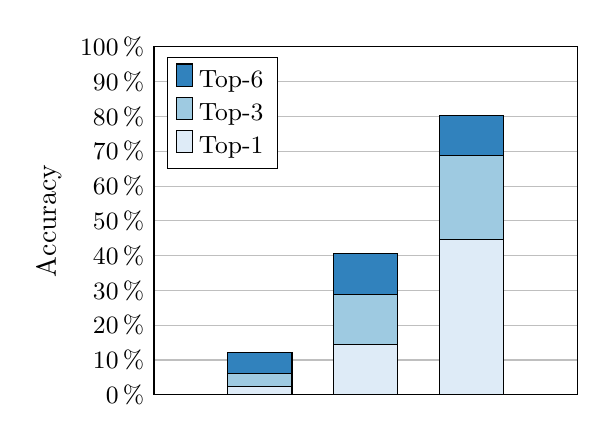
\begin{tikzpicture}
\begin{axis}[
  ybar stacked,
  % width=\linewidth,
  height=6cm,
  % title={Accuracy of Repair Template Prediction},
  ylabel={Accuracy},
  bar width=0.82cm,
  ymin=0.0,
  ymax=100.0,
  ytick={0.0, 10.0, 20.0, 30.0, 40.0, 50.0, 60.0, 70.0, 80.0, 90.0, 100.0},
  yticklabel={\pgfmathparse{\tick}\pgfmathprintnumber{\pgfmathresult}\,\%},
  ytick style={draw=none},
  ymajorgrids = true,
  symbolic x coords={random, popular, dnn},
  enlarge x limits=0.5,
  xtick=data,
  xtick style={draw=none},
  xticklabels={\random, \popular, \dnn},
  %x tick label style={rotate=45, anchor=north east},
  x tick label style={font=\small},
  y tick label style={font=\small},
  reverse legend,
  transpose legend,
  legend style={legend pos = north west, legend columns=4, font=\small},
]

\addplot[draw=black, fill=blue1] coordinates {(random, 2.35646958011996552) (popular, 14.438731790916881) (dnn, 44.64438731790917)};
\addlegendentry{Top-1}
\addplot[draw=black, fill=blue2] coordinates {(random, 3.6846615252784924) (popular, 14.395886889460153) (dnn, 24.250214224507282)};
\addlegendentry{Top-3}
\addplot[draw=black, fill=blue3] coordinates {(random, 6.212510711225363) (popular, 11.825192802056556) (dnn, 11.482433590402735)};
\addlegendentry{Top-6}

\end{axis}
\end{tikzpicture}
\caption{
  Results of our template prediction classifiers using the \emph{50 most
  popular} templates. We present the results up to the top 6 predictions, since
  our synthesis algorithm considers that many templates before falling to a
  different location.
}
\label{fig:accuracy-results}
\end{figure}


\begin{figure}[t]
  \centering
  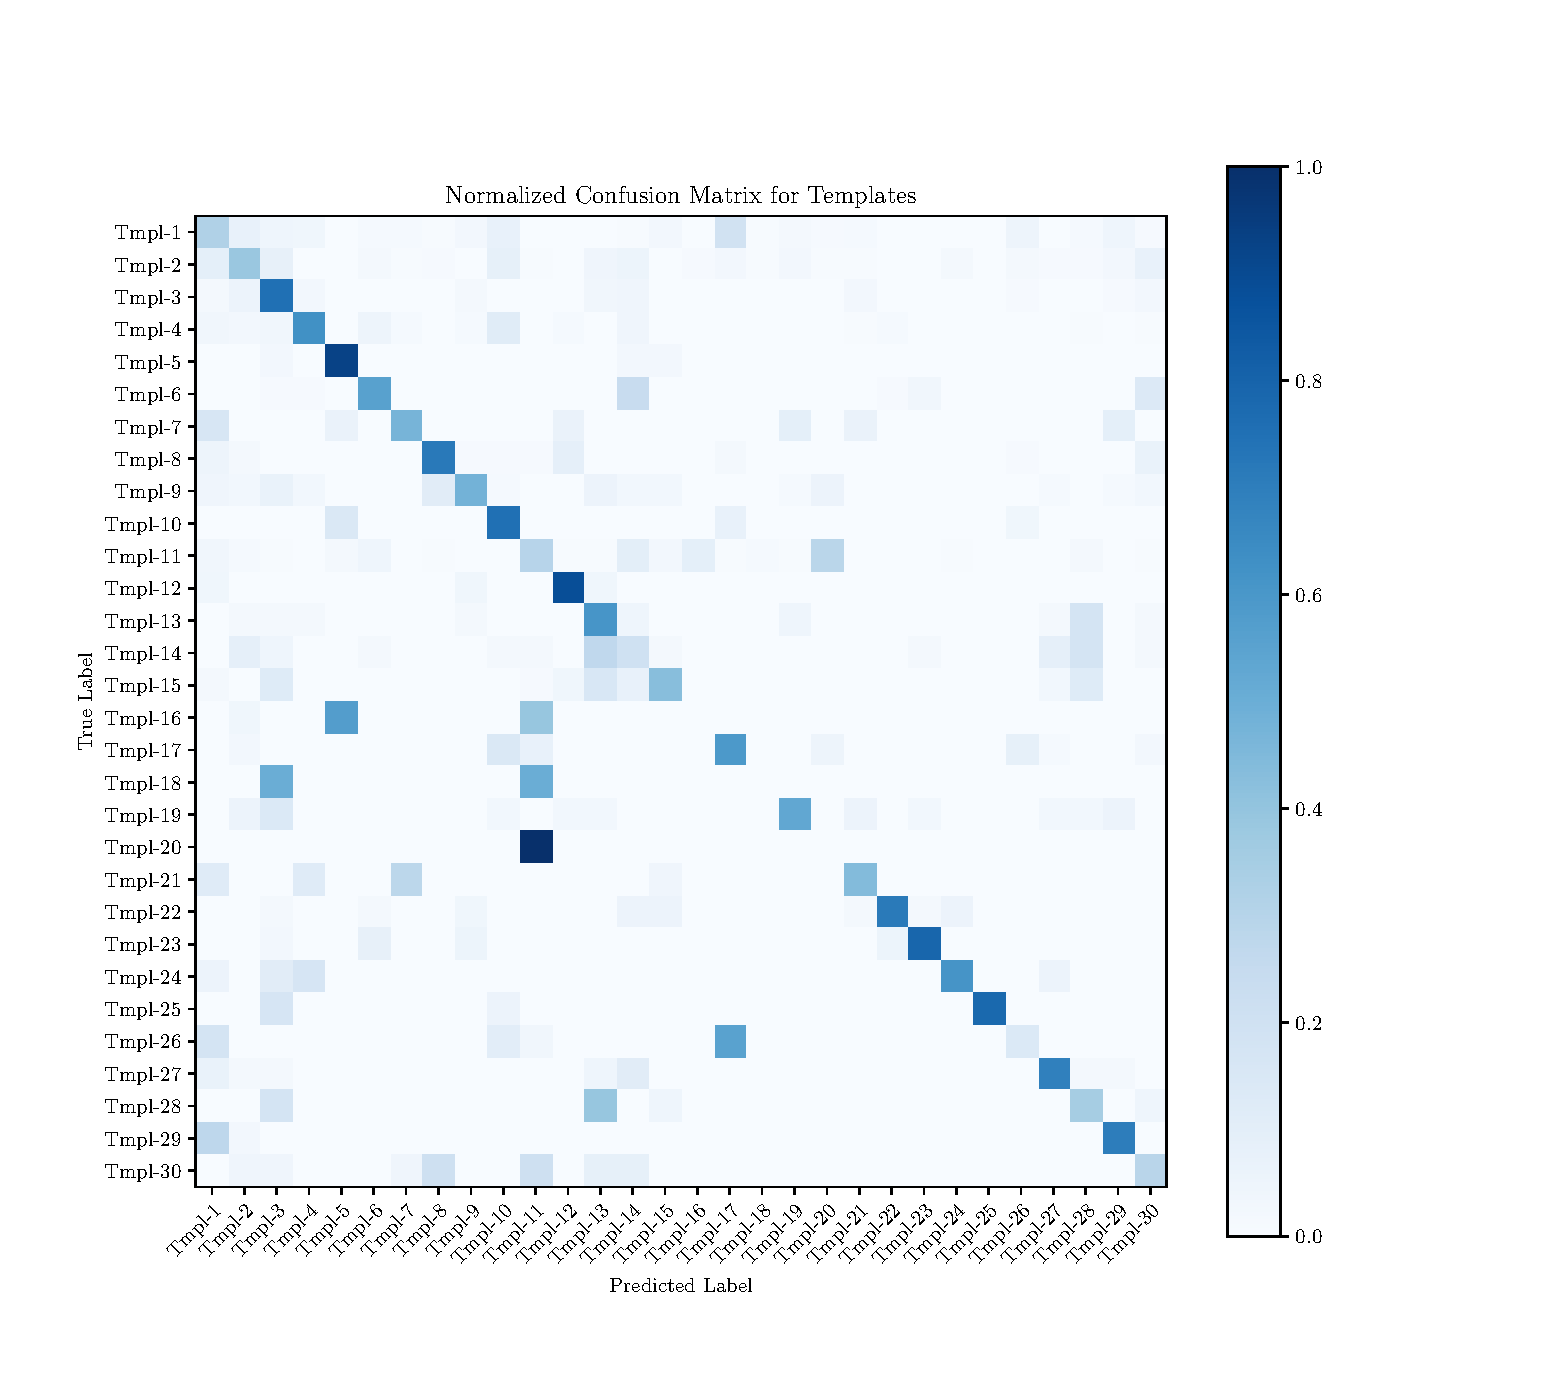
\includegraphics[trim={30 40 100 70},clip,height=2.2in]{evaluation-conf-matrix.pdf}
  \caption{The confusion matrix of the \emph{top 30} templates. Bolder parts of
  the heatmap show templates that are often mis-predicted with another template.
  The bolder the diagonal is, the more accurate predictions we make.}
  \label{fig:conf-matrix}
\end{figure}

\mypara{Results: Template ``Confusion''}
%
The \emph{confusion matrix} of the each location's top prediction shows which
templates our models mix up.
%
\autoref{fig:conf-matrix} shows this matrix for the top 30 templates acquired
from the \SPRING training set and were tested on the \FALL dataset.
%
Note that most templates are predicted correctly and only a few of them are
often mis-predicted for another template.
%
For example, we see that programs that require template 20
(\elet{\hat{z}}{\epcases{\hat{t}}{\hat{x}}{\hat{y}}{\hat{a}}}{\_}) to be fixed,
almost always are mis-predicted with template 11 (\elet{(\hat{x},
\hat{y})}{\hat{t}}{(\_,\ \_)}). We observe that these templates are still very
similar, with both of them having a top-level |let| that manipulates tuples
$\hat{t}$.

\begin{framed}
  \noindent \toolname's learns correlations between program features and repair
  templates, yielding almost \emph{2x higher} accuracy than the baseline; by
  abstracting programs into features, \toolname is able to \emph{generalize}
  across years and different kinds of programs.
\end{framed}


\subsection{RQ2: Efficiency}
\label{sec:eval:efficiency}
\label{subsec:eval:man_rep_qual_eval}

Next we evaluate the efficiency of \toolname by measuring how many programs it
is able to generate a (well-typed) repair for.
%
Recall that the repair synthesis algorithm is guided by the repair template
predictions.
%
To measure efficiency, we give the synthesizer \emph{90s} to compute a repair
and timeout otherwise. (In general the procedure is undecidable, and we
conjecture that a longer timeout will diminish the practical usability for
novices.)
%
We evaluate the efficiency of \toolname by comparing
it against a baseline \naive implementation that, given the predicted fix
location, attempts to synthesize a repair from the trivial ``hole'' template
$\_$.

\autoref{fig:rite_naive} shows the cumulative distribution function of
\toolname's and \naive's repair rates over their synthesis time. We observe that
using the predicted templates for synthesis allows \toolname to generate
type-correct repairs for almost 60\% of the programs in under 10 seconds, which
is nearly 10 points higher than the \naive baseline. We also observe that
\toolname manages to repair around 10\% more programs than \naive, almost
consistently when execution times where higher than 10 seconds.

\begin{framed}
  \noindent \toolname can generate type-correct repairs for the majority of
  ill-typed programs in under 10 seconds.
\end{framed}

% The 11.85\% of the programs that fail to be repaired within that amount of time
% fall in the case of the combined failure of our predictive models to give high
% confidence scores to the correct locations and templates, thus making synthesis
% very expensive.

% \begin{table}
%   \centering
%   \begin{tabular}{l|ccc}
%     Classifier & Completed & Repair Rate & Time (sec) \\
%     \hline
%     \naive   & 77.86\% & 74.78\% & 11.72 \\
%     \toolname & 88.15\% & 84.80\% & 8.81 \\
%   \end{tabular}
%   \caption{Experimental results of \toolname's synthesis.}
%   \label{tab:rite_naive}
% \end{table}

\begin{figure}
  \centering
  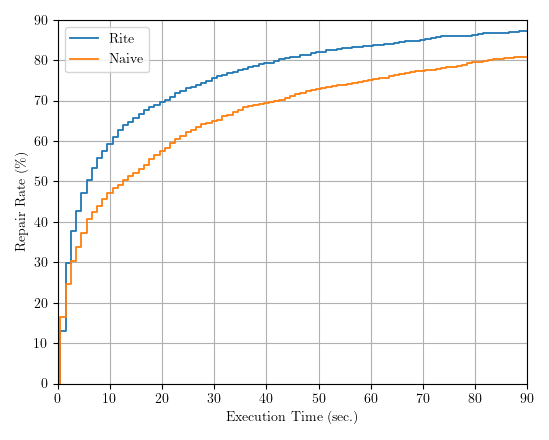
\includegraphics[height=2.4in]{cdf.png}
  \caption{Test set repair rate over execution time. Results are accumulated into 1 second intervals.}
  \label{fig:rite_naive}
\end{figure}

%%%%%%%%%%%%%%%%%%%%%%%%%%%%%%%%%%%%%%%%%%%%%%%%%%%%%%%%%%%%%%%%%%%%%%%%%%%%%%%
%%%%%%%%%%%%%%%%%%%%%%%%%%%%%%%%%%%%%%%%%%%%%%%%%%%%%%%%%%%%%%%%%%%%%%%%%%%%%%%
%%%%%%%%%%%%%%%%%%%%%%%%%%%%%%%%%%%%%%%%%%%%%%%%%%%%%%%%%%%%%%%%%%%%%%%%%%%%%%%
%%%%%%%%%%%%%%%%%%%%%%%%%%%%%%%%%%%%%%%%%%%%%%%%%%%%%%%%%%%%%%%%%%%%%%%%%%%%%%%

\subsection{RQ3: Usefulness}
\label{sec:eval:useful}

Finally, the ultimate proof of the pudding is in whether the repair-based
error messages generated by \toolname were actually useful to novices.
%
To assess the quality of \toolname's repairs, we conducted an online human
study with 29 participants.
%
Each participant was asked to evaluate the quality of the program fixes
and their locations against a state-of-the-art baseline
(\seminal ~\citep{Lerner2007-dt}).
%
For each program, beyond the two repairs, participants were presented
with the original ill-typed program, along with the standard \ocaml
compiler's error message and a short description of what the original
author of the program intended it to do.
%
From this study, we found that both the edit locations and final
repairs produced by \toolname were better than
\seminal's in a statistically significant manner.

\mypara{User Study Setup}
%
Study participants were recruited from two public research
institutes (names elided for DBR), and was advertised on Twitter.
%
Participants had to assess the quality of, and give comprehensible 
bug descriptions for, at least 5 / 10 stimuli. The study took around
25 minutes to complete. Participants were compensated by entering a 
drawing for an Amazon Echo voice assistant. There were 29 valid participants.
%
We created the stimuli by randomly selecting a corpus of 21 buggy programs
from the 1834 programs in our dataset where repairs were synthesized. 
%
From this corpus, each participant was shown 10 randomly-selected buggy 
programs, and two candidate repairs: one generated by \toolname and one 
by \seminal. 
%
For both algorithms, we used the highest-ranked solution returned. 
%
Participant were always unaware which tool generated which candidate 
patch. 
%
Participants were then asked to assess the quality of each
candidate repair on a Likert scale of 1 to 5 and were asked 
for a binary assessment of the quality of each repair's edit 
location.
%
We also collected self-reported estimates of both programming and
\ocaml-specific experience as well as qualitative data assessing factors
influencing each participant's subjective judgment of repair quality.
%
From the 29 participants, we collected 554 patch quality assessments, 
277 each for \toolname and \seminal generated repairs.

%\begin{figure}
%  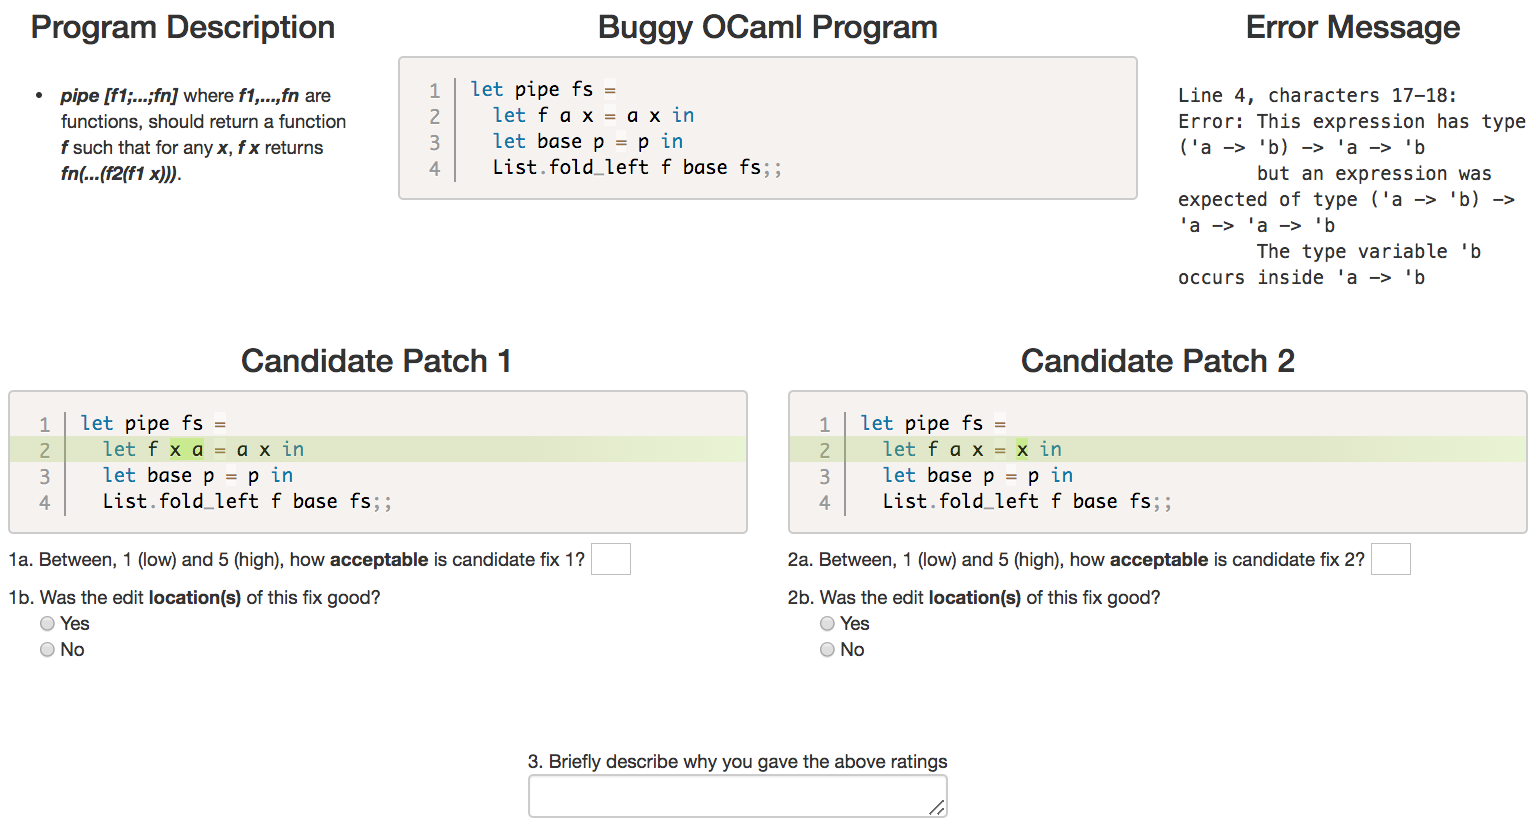
\includegraphics[width=8cm]{SampleStimuli.png}
%  \caption{A sample stimulus used for assessing repair quality.}
%  \label{fig:stimulus}
%\end{figure}

\mypara{Results}
%
In a statistically significant manner, humans perceive that
\toolname's fault localization and final repairs are both
of higher quality than those produced by \seminal ($p=0.030$
and $p=0.024$ respectively)~\footnote{All tests for statistical
significance used the Wilcoxon signed-rank test.}.
%
Regarding fault localization, we find that humans agreed
with \toolname-identified edit locations 81.6\% of the time
but only agreed with those of \seminal 74.0\% of the time.
%
% This 10\% increase is important because \ME{You should explain why this matters.}
%
As for the final repair, humans also prefer \toolname's patches
to those produced by \seminal. Specifically, \toolname's repairs
achieved an average quality rating of 2.41/5 while \seminal's
repairs had an average rating of only 2.11/5, a 14\% increase ($p=0.030$),
showing a statistically significant improvement over \seminal.

\begin{figure*}
\begin{subfigure}[t]{.33\textwidth}
\centering
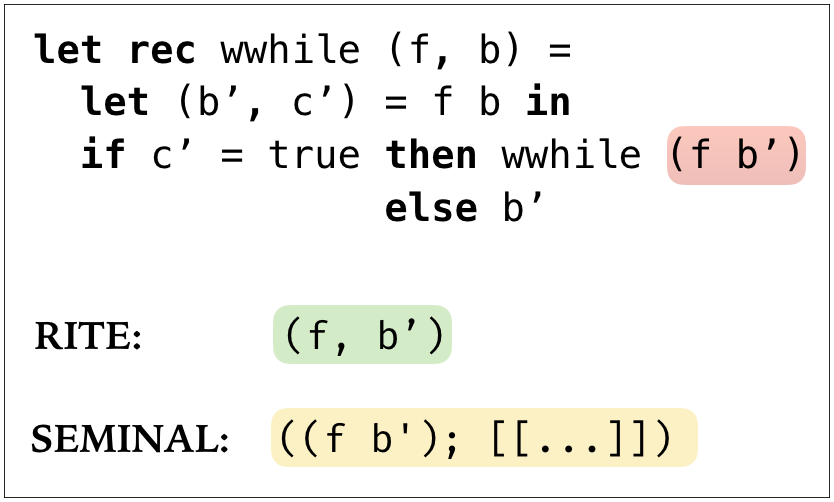
\includegraphics[height=1.4in]{comp1.png}
\caption{\toolname (4.5/5) better than \seminal(1.1/5) with 12 responses $p=0.002$.}
\label{subfig:good1}
\end{subfigure}
\begin{subfigure}[t]{.33\textwidth}
\centering
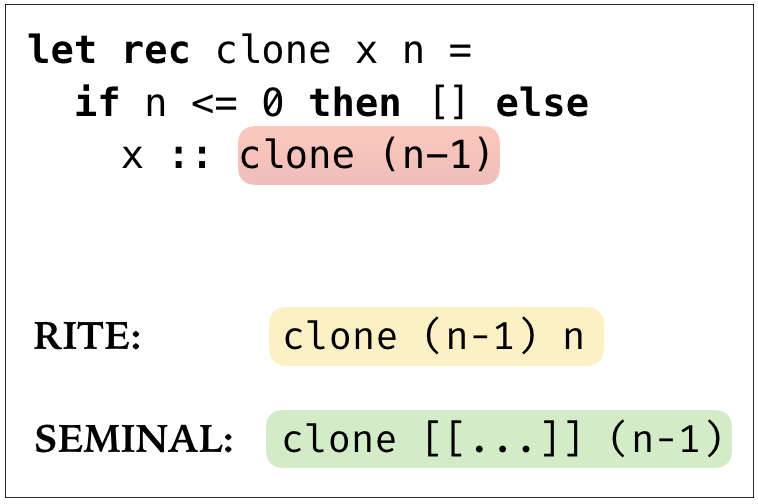
\includegraphics[height=1.4in]{comp2.png}
\caption{\toolname (1.5/5) worse than \seminal(4.1/5) with 18 responses $p=0.0002$.}
\label{subfig:bad}
\end{subfigure}
\begin{subfigure}[t]{.29\textwidth}
\centering
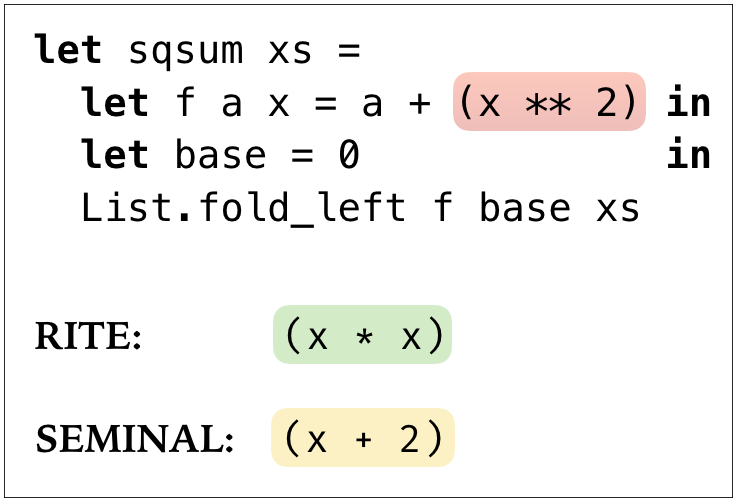
\includegraphics[height=1.4in]{comp3.png}
\caption{\toolname (4.8/5) better than \seminal(1.2/5) with 17 responses $p=0.0003$.}
\label{subfig:good2}
\end{subfigure}
\end{figure*}

\mypara{Qualitative Comparison}
%
We consider several case studies where there were
statistically-significant differences between
the human ratings for \toolname's and \seminal's
repairs.
%
The task in Figure~\ref{subfig:good1} is
\texttt{wwhile(f, b)} should return $x$ where
there exist values $v_0,...,v_n$ such that:
$b = v_0$, $x = v_n$, and for each $i$ between
0 and $n-2$, we have $f v_i = (v_i+1, true)$
and $f v_n-1 = (v_n, false)$.
%
The task in Figure~\ref{subfig:bad} is to
return a list of \texttt{n} copies of \texttt{x}.
%
The task in Figure~\ref{subfig:good2} is to
return the sum of the squares of the numbers
in the list \texttt{xs}.
%
Humans rated \toolname's repairs better
for the programs in Fig~\ref{subfig:good1}
and~\ref{subfig:good2}.
%
In both cases, \toolname's found a solution
which typechecks and conforms to the problem's
semantic specification.
%
\seminal, however, found a repair that was
either incomplete (\ref{subfig:good1}) or
semantically incorrect (\ref{subfig:good2}).
% FIXME: Add what good thing about \toolname caused this.
On the other hand, in ~\ref{subfig:bad}, \toolname
does worse as the \emph{second} parameter should
be \verb|n-1|. In fact, \toolname's second ranked
repair is the correct one, but it is equal
to the first in terms of edit distance.

\begin{framed}
\noindent Humans perceive both \toolname's edit locations
 and final repair quality to be better than those produced
 by \seminal, a state-of-the-art \ocaml repair tool, in a
 statistically-significant manner.
\end{framed}

\subsection{RQ4: Impact of Templates on Quality}

Finally, we seek to evaluate whether \toolname's template-guided
approach is really at the heart of its effectiveness. To do so,
as in \S~\ref{sec:eval:efficiency}, we performed a user study
to compare the results of using \toolname's error messages
synthesized from predicted templates to those generated by
a \naive synthesizer that returns the first well-typed term
(\ie synthesized from the trivial $\_$ template).

\mypara{User Study Setup}
%
For this user study, we reused the corpus of 21 buggy programs
randomly chosen in \S~\ref{sec:eval:useful}. For each of the
programs we generated three messages: using \toolname, using \seminal,
and using the \naive approach but at the \emph{same location} predicted
by \toolname. We then randomized and masked the order in which the tools'
messages were reported, and asked three experts (authors of this paper)
to rate the errors as one of Good, Ok or Bad.

\mypara{Results}
%
Figure~\ref{fig:comparison} summarizes the results of the rating.
%
Recall that each of 20 programs got 3 ratings, so there are a
total of 60 ratings per tool.
%
\toolname dominates with 22 Good, 20 Ok and 18 Bad ratings;
\seminal follows with only 12 Good, 11 Ok and 37 Bad; while
\naive received no Good scores, 12 Ok scores and a
dismal 48 Bad scores.
%
On average, with (Bad = 0, Ok = 0.5, Good = 1),
\toolname scored 0.53, \seminal 0.30, and \naive
just 0.1.
%
Our rating agreement kappa is 0.54, which is considered ``moderate agreement''.

\begin{framed}
  \noindent Repairs generated from predicted
  templates were of significantly higher quality
  than those from expert-biased enumeration (\seminal)
  or \naive type-directed enumeration.
\end{framed}

\begin{figure}[t]
  \centering
  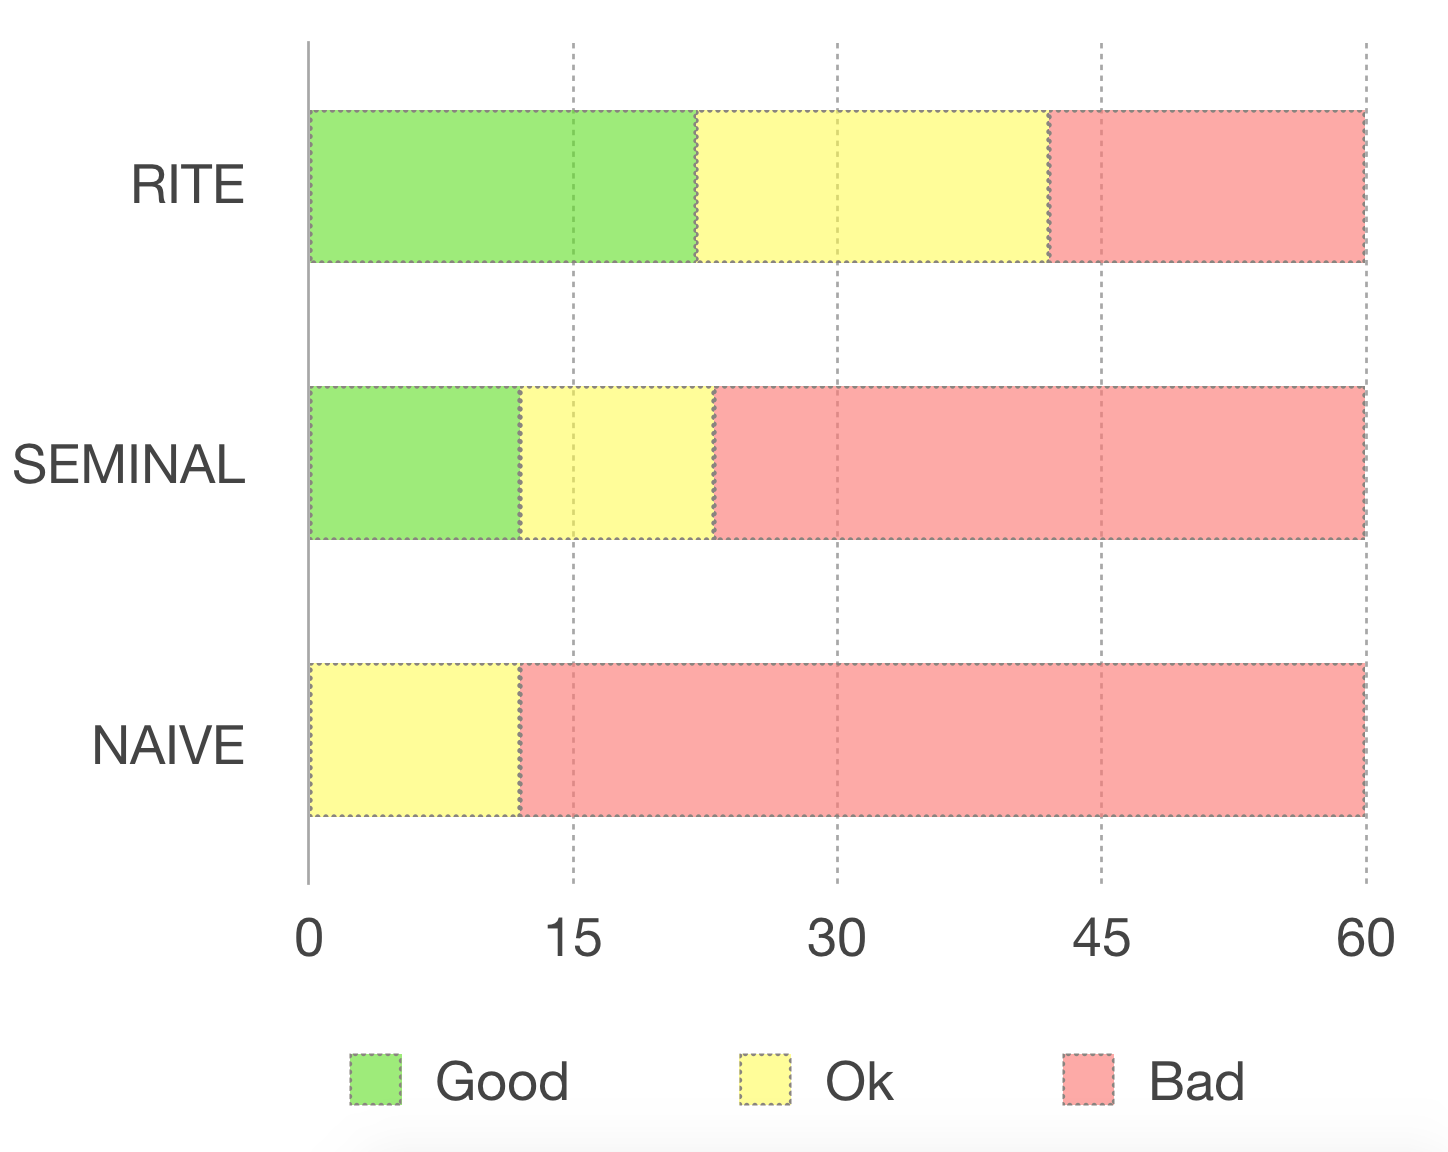
\includegraphics[height=1.5in]{comparison.png}
  \caption{Rating the errors generated by \toolname, \seminal and \naive enumeration.}
  \label{fig:comparison}
\end{figure}
